\documentclass[12pt]{article}
\usepackage{graphicx}
\usepackage{wrapfig}
\usepackage{amsmath}
\usepackage[brazil]{babel}
\usepackage[a4paper, left=3cm, top=3cm, right=2cm, bottom=2cm]{geometry}
\usepackage{float}
\usepackage{hyperref}
\usepackage[square,numbers]{natbib}
\bibliographystyle{abbrvnat}

\setcounter{secnumdepth}{4}  % Permite numerar até nível 4
\setcounter{tocdepth}{4}     % Inclui nível 4 no sumário

\newcommand{\subsubsubsection}[1]{%
  \paragraph{#1}\mbox{}\\
}

\begin{document}


\begin{titlepage}
    \begin{center}
        Universidade Federal de Santa Catarina\\
        Departamento de Engenharias da Mobilidade \\ Eletrônica Análogica - EMB5116\\

        \vspace{1.5cm}
        
\includegraphics[width=0.28\textwidth]{./images/vertical_sigla_fundo_claro.png}

        \vspace*{1.5cm}
        \fontsize{12pt}{16pt}\textbf{Eletrônica Analógica - Trabalho 2}

        \vspace*{1.5cm}
        Dr. Prof. Milton Evangelista de Oliveira Filhos

        \vspace*{1.0cm}
        \begin{tabular}{c c}
                André Stein - 22201053\\
                Danilo Machado - 22203056\\
                Pedro Lauxen - 22201064\\
        \end{tabular}

        \vspace*{\fill}
        {Joinville\\
        2025}
    \end{center}
\end{titlepage}


\tableofcontents\renewcommand*\contentsname{Sumário}
\newpage

\section{Introdução}

    Dispositivos transistores são utilizados comumente como meios de amplificar, ou chavear um circuito, de forma que o mesmo opere da maneira desejada no circuito. Dentre os transistores existentes os tipos mais comuns são os bipolares de junção,cujo são componentes formados pela junção de semicondutores,de forma que os agregando em conjuntos do tipo NPN ou PNP, forma-se um dispositivo que opera conforme é configurada sua polarização, porém assim como há a existência de componentes específicos dentro do mundo dos capacitores e resistores, dentro do mundo dos transistores existem os transistores de efeito de campo, que utilizam outra forma de controlar o fluxo de corrente por semicondutores. Neste trabalho serão descritos diferentes transistores de efeito de campo(FET) como,FET de junção (JFET),FET de Metal-Óxido-Semicondutor(MOSFET) e por último o Transistor Bipolar de Porta Isolada(IGBT) determinando como funciona cada um desses componentes, assim como será feita a comparação entre os mesmos, e por fim a comparação direta com transistores bipolares de junção.

\newpage

\section{Transistores de Efeito de Campo}

\section{FET de junção(JFET)}

O transistor de efeito de campo de junção, conhecido com JFET, é um dos dispositivos semicondutores mais importantes na eletrônica analógica. Ele opera a partir do controle do fluxo de portadores de carga em um canal semicondutor através de um campo elétrico aplicado a uma junção PN. Ao contrário do transistor bipolar (BJT), o JFET é controlado por tensão, o que confere ao dispositivo alta impedância de entrada e baixo consumo de energia, assim o JFET não carrega o circuito anterior, sendo ideal como estágio de entrada em amplificadores.

        \begin{figure}[htpb!]
            \centering
            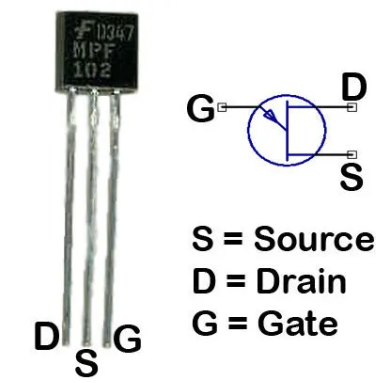
\includegraphics[width=0.3\linewidth]{images/Captura de tela 2025-10-18 223003.png}
            \caption{Transistor JFET}
        \end{figure}

\subsection{Histórico do Transistor JFET}

 Sua concepção teórica foi inicialmente proposta em 1928 por Julius Edgar Lilienfeld, que descreveu o princípio de controle de corrente por meio de um campo elétrico aplicado a um semicondutor. No entanto, na época, as limitações tecnológicas relacionadas à pureza dos materiais semicondutores e à ausência de técnicas avançadas de fabricação impediram a implementação prática do dispositivo.

Somente a partir da década de 1950, com o avanço dos processos de dopagem e crescimento controlado de cristais de silício e germânio, tornou-se possível fabricar JFETs funcionais. Empresas como a Bell Labs e a Fairchild Semiconductor tiveram papel fundamental no aperfeiçoamento da tecnologia. O JFET tornou-se, o primeiro tipo de transistor de efeito de campo fabricado, antecedendo os MOSFETs.


\subsection{Princípio de Funcionamento}


O JFET é um dispositivo semicondutor de três terminais: Gate (G), Source (S) e Drain (D). Seu funcionamento baseia-se no controle do fluxo de portadores de carga através de um canal semicondutor (de tipo N ou P), que é modulado pela tensão aplicada entre o gate e a fonte. 

\begin{itemize}
    \item \textbf{Gate (G) — Porta:} É o terminal responsável pelo controle do fluxo de corrente no canal. 
    O gate é formado por uma junção PN polarizada reversamente em relação ao canal, o que faz com que praticamente não haja corrente fluindo pelo gate. 
    A tensão aplicada entre o gate e a fonte ($V_{GS}$) cria um campo elétrico que modula a largura efetiva do canal, controlando assim a corrente que circula entre o dreno e a fonte.

    \item \textbf{Source (S) — Fonte:} É o terminal por onde os portadores de carga entram no canal. 
    Para um JFET de canal N, os portadores são elétrons; para um JFET de canal P, são lacunas. 
    A tensão do gate é sempre medida em relação à fonte ($V_{GS}$), tornando o \textit{source} o terminal de referência para o controle do dispositivo.

    \item \textbf{Drain (D) — Dreno:} É o terminal por onde os portadores de carga saem do canal após percorrê-lo. 
    A corrente que flui do dreno para a fonte ($I_D$) depende da tensão $V_{GS}$ aplicada ao gate e da tensão $V_{DS}$ aplicada entre o dreno e a fonte. 
    Quando $V_{GS}$ se torna mais negativo (no caso de um JFET de canal N), a região de depleção se expande, estreitando o canal e reduzindo a corrente $I_D$, até o ponto de corte (pinch-off).
\end{itemize}

        \begin{figure}[htpb!]
            \centering
            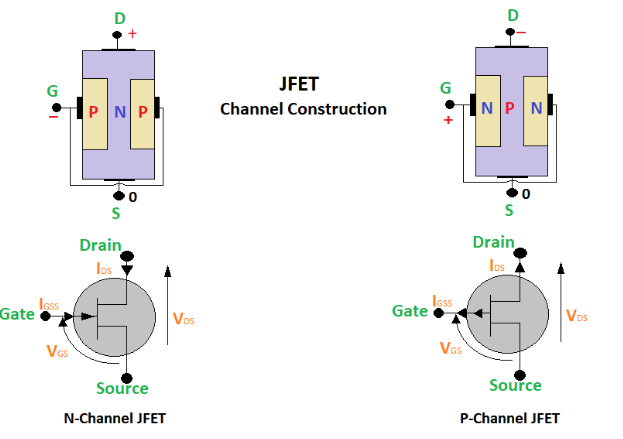
\includegraphics[width=0.8\linewidth]{images/pn.png}
            \caption{Representação de um JFET}
        \end{figure}
                
\subsubsection{Fluxo de Corrente no Canal}

Quando uma tensão \(V_{DS}\) é aplicada entre o dreno e a fonte, uma corrente \(I_D\) começa a fluir através do canal, composta por elétrons (no JFET de canal N) ou lacunas (no JFET de canal P). A magnitude dessa corrente depende da largura efetiva do canal condutor.

O gate é uma junção PN polarizada reversamente. Isso significa que praticamente não há corrente de gate, pois a barreira de potencial impede o fluxo de portadores. Entretanto, a região de depleção da junção se expande, reduzindo a seção transversal do canal e, consequentemente, controlando a corrente \(I_D\).


        \begin{figure}[htpb!]
            \centering
            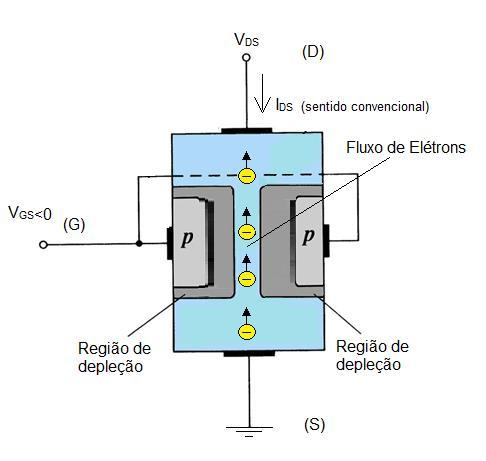
\includegraphics[width=0.5\linewidth]{images/JFET-de-canal-n-reversamente-polarizado-corpo-com-cargas-negativas-nas-proximidades-da.png}
            \caption{JFET de canal n reversamente polarizado}
            \label{fig:JFET}
        \end{figure}
                
\subsubsection{Efeito da Polarização do Gate}

O gate é constituído por uma junção PN polarizada reversamente em relação ao canal. Nessa condição, praticamente não há corrente fluindo pelo gate, pois a barreira de potencial da junção impede o movimento de portadores de carga. Apesar disso, a polarização reversa provoca o alargamento da região de depleção, que se estende lateralmente a partir das junções PN em direção ao interior do canal.

À medida que a tensão $V_{GS}$ (tensão entre gate e source) se torna mais negativa no caso de um JFET de canal N, a região de depleção se expande, reduzindo a largura efetiva do canal condutor. Com a diminuição dessa seção transversal, a resistência do canal aumenta, resultando em uma diminuição da corrente $I_D$. Esse mecanismo de controle é o que caracteriza o funcionamento do JFET como um dispositivo de efeito de campo, o campo elétrico gerado pela tensão no gate modula a condutância do canal.

        \begin{figure}[htpb!]
            \centering
            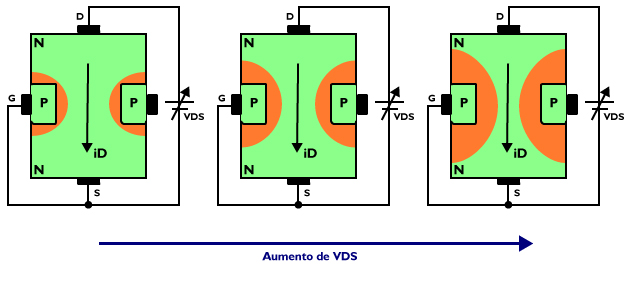
\includegraphics[width=0.8\linewidth]{images/aumento Vds.png}
            \caption{Representação da região de depleção}
        \end{figure}

\subsubsection{Equação de Shockley}

A característica fundamental do JFET é o controle da corrente do canal por meio do campo elétrico estabelecido pela tensão \(V_{GS}\).  
Para um JFET de canal N:
\begin{itemize}
    \item Quando \(V_{GS} = 0\), o canal apresenta sua máxima condutividade, e a corrente \(I_D\) atinge o valor máximo \(I_{DSS}\).
    
    \item À medida que \(V_{GS}\) torna-se negativo, as regiões de depleção em torno do gate aumentam, estreitando o canal e reduzindo \(I_D\).
    
    \item Quando \(V_{GS}\) atinge a tensão de corte \(V_P\), o canal é completamente bloqueado, e \(I_D \approx 0\).
\end{itemize}

Esse comportamento é representado pela Equação de Shockley:
\[
I_D = I_{DSS} \left( 1 - \frac{V_{GS}}{V_P} \right)^2
\]

\subsubsection{Regiões de Operação}

Para o transistor JFET pode-se distinguir três regiões principais de operação:

\begin{enumerate}
    \item \textbf{Região ôhmica (ou linear):} 
    Quando $V_{DS}$ é pequeno, a corrente $I_D$ é aproximadamente proporcional à tensão $V_{DS}$, obedecendo uma relação quase linear. O dispositivo atua como um resistor controlado por tensão, e o canal permanece totalmente aberto.

    \item \textbf{Região de saturação (ou ativa):} 
    À medida que $V_{DS}$ aumenta, a tensão no dreno se torna mais positiva em relação ao gate, fazendo com que a região de depleção se expanda mais próxima ao dreno do que ao source. 
    Em um ponto específico, conhecido como tensão de estrangulamento ou pinch-off ($V_P$), as regiões de depleção provenientes das laterais do canal se encontram, estrangulando-o. 
    A partir desse ponto, o aumento de $V_{DS}$ não causa um aumento significativo em $I_D$, e a corrente se torna praticamente constante. 
    O JFET opera, então, como uma fonte de corrente controlada por tensão.

    \item \textbf{Região de corte:} 
    Quando $V_{GS}$ é suficientemente negativo (em módulo igual ou superior a $V_P$), o canal é completamente bloqueado pela expansão das regiões de depleção, impedindo o fluxo de corrente. Nessa condição, $I_D$ é aproximadamnete 0.
\end{enumerate}

        \begin{figure}[htpb!]
            \centering
            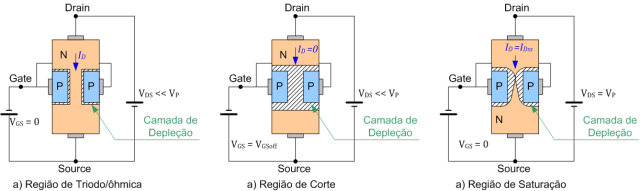
\includegraphics[width=1.0\linewidth]{images/regioes.png}
            \caption{Representação de cada região}
        \end{figure}


\subsection{Construção e Design do JFET}

\subsubsection{Estrutura Física}

O JFET é construído a partir de um cristal semicondutor (geralmente silício) no qual se define um canal condutor de tipo N ou tipo P. O canal é cercado por regiões de dopagem oposta, que formam junções PN com o canal, conhecidas como regiões de gate. Como pode ser notado na  figura \ref{fig:JFET}.

Características da estrutura física:

\begin{itemize}
    \item \textbf{Canal semicondutor:} É levemente dopado para permitir controle eficaz da corrente, mantendo o valor de \(I_{DSS}\) dentro das especificações. O canal é formado longitudinalmente entre os terminais source e drain.


    \item \textbf{Junções Gate-Canal:} As regiões de dopagem do gate são fortemente dopadas para formar junções PN eficientes. A polarização reversa dessas junções controla a largura efetiva do canal.
    
    \item \textbf{Terminais Source e Drain:} Conectados nas extremidades do canal, permitem a entrada e saída de portadores de carga. 
    
    \item \textbf{Substrato:} Pode estar conectado ao gate (common gate) ou flutuante, dependendo do design. Em alguns casos, o substrato é de tipo oposto ao canal e atua como um dissipador térmico e suporte mecânico.
\end{itemize}

\subsubsection{Considerações de Dopagem e Materiais}

O controle da dopagem é crítico no projeto de JFETs, pois determina parâmetros elétricos essenciais:

\begin{itemize}
    \item Dopagem do canal: Uma dopagem mais leve aumenta a resistência do canal e permite maior controle da corrente pelo gate, mas reduz \(I_{DSS}\).
    
    \item Dopagem do gate: Alta dopagem assegura junções PN de baixa resistência e pequena capacitância reversa, fundamental para alta frequência.
    
    \item Material semicondutor: Silício é predominante, mas arseneto de gálio (GaAs) é usado em JFETs de RF devido à maior mobilidade de elétrons e menor ruído.
\end{itemize}

\subsubsection{Geometria do Canal}

A geometria do canal é um dos fatores mais críticos no projeto de um JFET, influenciando diretamente o comportamento elétrico, térmico e a linearidade do dispositivo. O canal é caracterizado principalmente pelo seu comprimento \(L\), largura \(W\) e espessura \(t\), além do perfil de dopagem.

A geometria do canal determina diretamente os parâmetros elétricos fundamentais, como \(I_{DSS}\), \(V_P\), \(g_m\), linearidade, resposta em frequência e dissipação térmica. O projeto exige um equilíbrio cuidadoso entre largura, comprimento, espessura e dopagem para atender às especificações do circuito.

\subsubsubsection{Comprimento do Canal (\(L\))}

O comprimento do canal, medido entre os terminais source e drain impactam:

\begin{itemize}
    \item \textbf{Resistência do canal:} Um canal mais longo aumenta a resistência ôhmica \(R_{DS(on)}\), reduzindo a corrente máxima \(I_{DSS}\). A relação aproximada é \((R \propto L)/W\), considerando dopagem uniforme.
    
    \item \textbf{Linearidade em pequenos sinais:} Canais longos distribuem melhor o campo elétrico, reduzindo a distorção harmônica em amplificadores de baixa tensão.

    \item \textbf{Controle do pinch-off:} Comprimentos maiores tornam a transição entre a região ôhmica e a saturação mais suave, melhorando o controle da corrente.
    
    \item \textbf{Efeito de capacitâncias parasitas:} Canais longos podem aumentar a capacitância gate-drain \(C_{GD}\), afetando a resposta em alta frequência.
\end{itemize}

\subsubsubsection{Largura do Canal (\(W\))}

A largura do canal afeta:

\begin{itemize}
    \item \textbf{Corrente máxima:} Quanto maior a largura, maior a área condutora disponível, portanto maior \(I_{DSS}\).
    \item \textbf{Distribuição da densidade de corrente:} Canais muito estreitos podem concentrar a densidade de corrente, gerando aquecimento localizado e instabilidade térmica.
    \item \textbf{Sensibilidade à tensão do gate:} Larguras menores tornam o dispositivo mais sensível a variações de \(V_{GS}\), pois a região de depleção ocupa uma fração maior do canal.
\end{itemize}

\subsubsubsection{Espessura e Perfil de Dopagem do Canal}

A espessura efetiva do canal e o perfil de dopagem influenciam:

\begin{itemize}
    \item \textbf{Resistência de condução:} Canais mais finos ou menos dopados aumentam a resistência e reduzem \(I_{DSS}\), mas melhoram a linearidade.
    
    \item \textbf{Uniformidade do campo elétrico:} Perfis de dopagem gradientes permitem uma variação controlada da resistência ao longo do canal, suavizando o efeito de pinch-off.
    
    \item \textbf{Ruído térmico:} Canais finos geram menos corrente de ruído, essencial em aplicações de instrumentação de precisão.
\end{itemize}

\subsubsubsection{Relação Largura/Comprimento (\(W/L\))}

A razão \(W/L\) é frequentemente usada como parâmetro de projeto:

\begin{itemize}
    \item \textbf{Alta \(W/L\):} Favorece alta corrente \(I_{DSS}\) e menor resistência do canal, mas pode aumentar capacitâncias parasitas e reduzir linearidade.
    
    \item \textbf{Baixa \(W/L\):} Melhora linearidade e controle de corrente, mas limita \(I_{DSS}\) e aumenta a resistência.
\end{itemize}

Essas técnicas tornam os JFETs adequados para instrumentação, áudio de alta fidelidade e circuitos analógicos de precisão.

\subsection{Aplicações dos Transistores JFET}

\subsubsection{Amplificadores de Baixo Ruído}

Devido à sua alta impedância de entrada e baixo ruído térmico, os JFETs são amplamente usados em:

\begin{itemize}
    \item \textbf{Pré-amplificadores de microfone:} Mantêm a integridade do sinal e minimizam a interferência de ruído da fonte de sinal.
    
    \item \textbf{Amplificadores de instrumentação:} Em sistemas de medição de sinais muito pequenos, como sensores de temperatura ou tensão de strain gauge.
    
    \item \textbf{Amplificadores de áudio de alta fidelidade:} Garantem mínima distorção e preservação do espectro sonoro.
\end{itemize}

\subsubsection{Circuitos de Entrada de Instrumentação}

A elevada impedância de entrada torna o JFET ideal para circuitos onde a carga do sinal deve ser mínima:

\begin{itemize}
    \item \textbf{Osciloscópios e voltímetros de alta impedância:} Evitam carregamento do circuito sob teste.
    
    \item \textbf{Buffers (source followers):} Isolam estágios sensíveis, mantendo a amplitude e forma do sinal.
    
    \item \textbf{Amplificadores diferenciais de precisão:} Reduzem o erro devido a correntes de polarização.
\end{itemize}

\subsubsection{Fontes de Corrente Constante e Circuitos de Controle}

O JFET, em região de saturação, atua como uma fonte de corrente controlada por tensão:

\begin{itemize}
    \item \textbf{Fontes de corrente constantes:} Usadas em circuitos de polarização de transistores bipolares ou MOSFETs, proporcionando estabilidade térmica.
    
    \item \textbf{Circuitos de referência de corrente:} Mantêm corrente estável independentemente da tensão de alimentação.
    
    \item \textbf{Cascodes e espelhos de corrente:} Melhoram a faixa de ganho e a linearidade.
\end{itemize}

\subsubsection{Chaves Eletrônicas e Comutação Analógica}

JFETs são excelentes para chaves analógicas devido à baixa resistência de canal em região ôhmica:

\begin{itemize}
    \item \textbf{Multiplexadores analógicos:} Selecionam sinais sem degradar a amplitude ou forma de onda.
    
    \item \textbf{Chaves de áudio de alta fidelidade:} Evitam distorção em equipamentos de som profissional.
    
    \item \textbf{Amostragem de sinais:} Aplicações em conversores A/D e circuitos de medição.
\end{itemize}

\subsubsection{Circuitos de Alta Frequência e RF}

Apesar de não serem tão rápidos quanto MOSFETs de efeito de campo de óxido, JFETs são usados em RF devido à baixa capacitância de entrada:

\begin{itemize}
    \item \textbf{Osciladores de RF:} Estabilidade de frequência e baixo ruído.
    
    \item \textbf{Amplificadores de RF de baixo nível:} Como primeiros estágios em receptores de rádio e TV.
    
    \item \textbf{Misturadores e moduladores:} Precisão em circuitos de comunicação analógica.
\end{itemize}

\subsubsection{Aplicações em Sensores e Circuitos de Precisão}

O JFET é ideal em sensores devido à sua estabilidade e baixa corrente de fuga:

\begin{itemize}
    \item \textbf{Sensores de capacitância ou piezoelétricos:} O JFET não descarrega o sinal detectado.
    
    \item \textbf{Medidores de carga ou fotodiodos:} Minimiza corrente de polarização de entrada.
    
    \item \textbf{Amplificadores de instrumentação médica:} Eletrocardiogramas (ECG) e eletroencefalogramas (EEG).
\end{itemize}

\subsubsection{Outras Aplicações Especiais}

\begin{itemize}
    \item \textbf{Circuitos de proteção:} Limitadores de corrente em linhas sensíveis.
    \item \textbf{Modulação de sinais:} Em moduladores analógicos de amplitude ou frequência.
    \item \textbf{Pré-amplificadores de imagem e vídeo:} Onde baixa corrente de entrada e alta linearidade são essenciais.
    \item \textbf{Amplificadores operacionais JFET:} Amplificadores integrados com alto ganho e baixa corrente de bias.
\end{itemize}


\subsection{Comparação entre JFET e Transistor Bipolar (BJT)}

A seguir, são apresentadas as principais diferenças entre o JFET e o BJT, destacando aspectos de controle, impedância, ruído, estabilidade e faixa de frequência.

\begin{itemize}
    \item \textbf{Tipo de Controle:} 
    \begin{itemize}
        \item JFET: Controlado por tensão (\(V_{GS}\)), resultando em menor consumo de energia e mínima corrente de entrada.
        \item BJT: Controlado por corrente (\(I_B\)), exigindo corrente de base para operar.
    \end{itemize}

    \item \textbf{Impedância de Entrada:} 
    \begin{itemize}
        \item JFET: Impedância de entrada muito alta, da ordem de megaohms ou superior, evitando carregamento do circuito anterior.
        \item BJT: Impedância de entrada relativamente baixa, limitada pela base, o que pode afetar estágios sensíveis de sinal.
    \end{itemize}

    \item \textbf{Ruído e Estabilidade:} 
    \begin{itemize}
        \item JFET: Apresenta menor ruído de entrada e maior estabilidade térmica, ideal para instrumentação e aplicações de precisão.
        \item BJT: Maior ganho de corrente, mas sensível à variação térmica; preferido em estágios de potência e amplificação de sinais maiores.
    \end{itemize}

    \item \textbf{Faixa de Frequência:} 
    \begin{itemize}
        \item JFET: Pode operar em frequências elevadas, adequado para circuitos de RF de baixo nível.
        \item BJT: Mais eficiente em altas potências de RF, devido à maior mobilidade de portadores e capacidade de conduzir correntes mais elevadas.
    \end{itemize}
\end{itemize}


\section{FET de Metal-Óxido-Semicondutor(MOSFET)}

        \begin{figure}[htpb!]
            
            \centering
            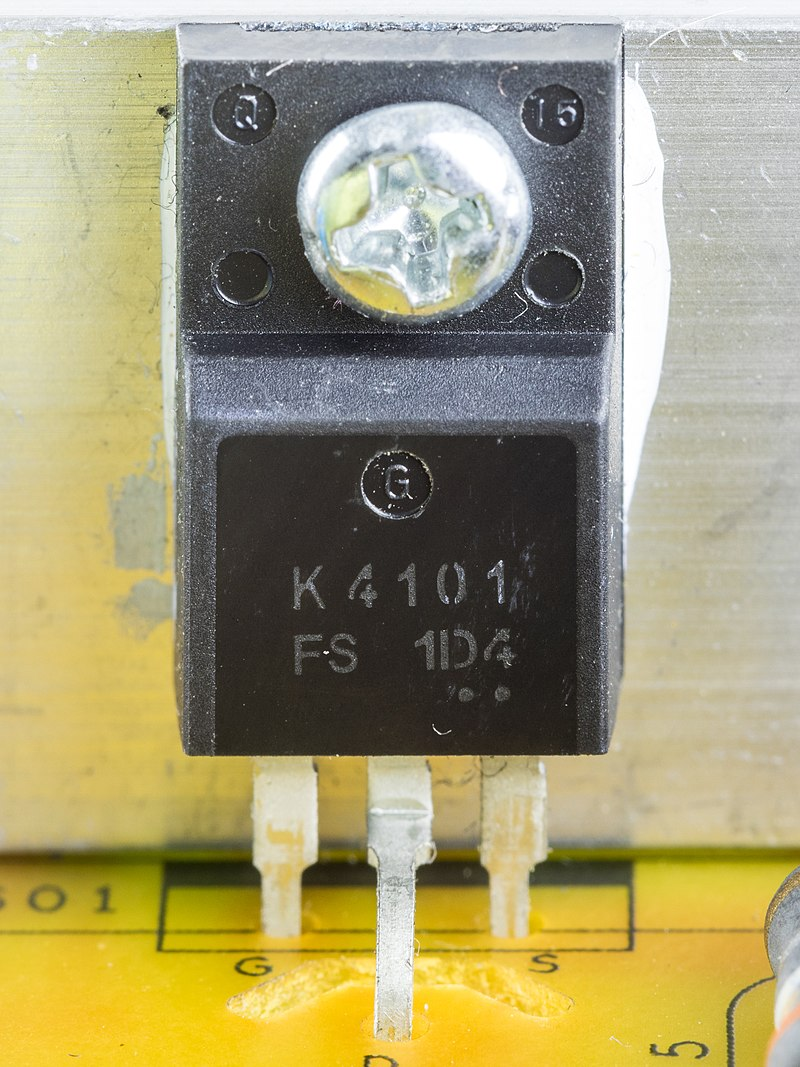
\includegraphics[width=0.2\textwidth]{./images/Dell_Professional_P2212H_-_power_supply_board_-_K4101FS-2149.jpg}
            \caption{MOSFET de potência.} 

        \end{figure}

    O transistor MOSFET (acrônimo de Metal Oxide Semiconductor Field Effect Transistor, ou transistor de efeito de campo semicondutor de óxido metálico — TECMOS), é o tipo mais comum de transístores de efeito de campo em circuitos tanto digitais quanto analógicos. Seu princípio básico foi proposto pela primeira vez por Julius Edgar Lilienfeld, em 1925. 

    Os transistores de efeito de campo diferentemente dos transistores bipolares comuns são típicos amplificadores de tensão e não de corrente. Enquanto a corrente de coletor de um transistor comum é função da corrente de base, num transistor de efeito de campo, a corrente de dreno é função da tensão de comporta, conforme indica a figura \ref{fig:comparacao}.

        \begin{figure}[htpb!]
            
            \centering
            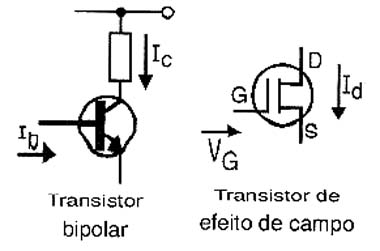
\includegraphics[width=0.4\textwidth]{./images/transisCampo.jpg}
            \caption{comparação entre transistor bipolar e transistor de efeito de campo.}
            \label{fig:comparacao}

        \end{figure}

        \begin{figure}[htpb!]
            
            \centering
            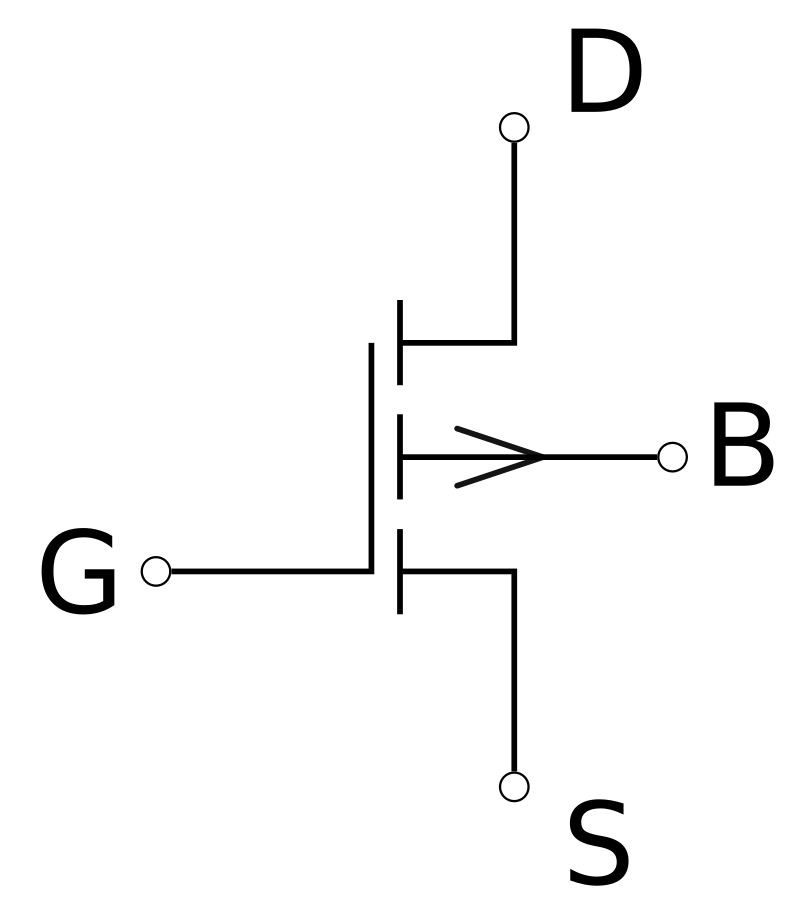
\includegraphics[width=0.2\textwidth]{./images/Mosfet-wp.svg.png}
            \caption{Símbolo de esquema elétrico de um MOSFET.}

        \end{figure}
        
        Uma fina película de óxido de metal isola a região de comporta da região do canal que liga o dreno à fonte. Isso faz com que a impedância de entrada do MOSFET seja muito alta, o que significa que ele consome muito pouca corrente da fonte de sinal que está dirigindo a comporta. Essa característica torna os MOSFETs ideais para circuitos de alta impedância, como amplificadores de áudio e circuitos digitais. Além disso, os MOSFETs são capazes de operar em frequências muito altas, tornando-os adequados para aplicações em rádio frequência (RF) e micro-ondas.

        \begin{figure}[htpb!]
            
            \centering
            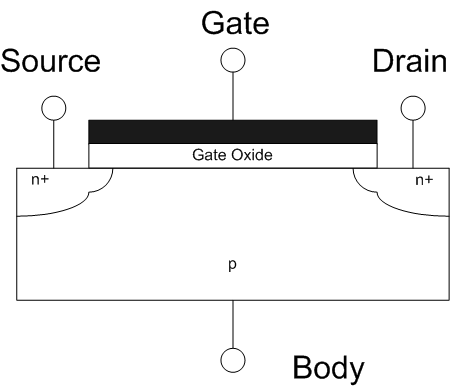
\includegraphics[width=0.3\textwidth]{./images/FET_cross_section.png}
            \caption{Símbolo de esquema elétrico de um MOSFET.}

        \end{figure}



        A palavra "metal" no nome é um anacronismo vindo dos primeiros chips, onde as comportas (gates) eram de metal. Os chips modernos usam comportas de polissilício, mas ainda são chamados de MOSFETs. Um MOSFET é composto de um canal de material semicondutor de tipo N ou de tipo P e é chamado respectivamente de NMOS ou PMOS. Geralmente o semicondutor escolhido é o silício, mas alguns fabricantes, principalmente a IBM, começaram a usar uma mistura de silício e germânio (SiGe) nos canais dos MOSFETs. Infelizmente muitos semicondutores com melhores propriedades elétricas do que o silício, tais como o arsenieto de gálio, não formam bons óxidos nas comportas e portanto não são adequados para os MOSFETs. O IGFET é um termo relacionado que significa Insulated-Gate Field Effect Transistor, e é quase sinônimo de MOSFET, embora ele possa se referir a um FET com comporta isolada por um isolante não óxido.

        O terminal de comporta é uma camada de polissilício (sílicio policristalino) colocada sobre o canal, mas separada do canal por uma fina camada de dióxido de silício isolante. Quando uma tensão é aplicada entre os terminais comporta (gate) e fonte (source), o campo elétrico gerado penetra através do óxido e cria uma espécie de "canal invertido" no canal original abaixo dele. O canal invertido é do mesmo tipo P ou tipo N, como o da fonte ou do dreno, assim, ele cria um condutor através do qual a corrente elétrica possa passar. Variando-se a tensão entre a comporta e a fonte se modula a condutividade dessa camada e torna possível se controlar o fluxo de corrente entre o dreno e a fonte. Existem também modelos de Amplificador operacional baseados na tecnologia FET/MOSFET, muito úteis e com grande utilização na indústria eletrônica.




\section{Transistor Bipolar de Porta Isolada(IGBT)}

    O tipo de transistor IGBT, pode ser definido de maneira técnica como um transistor formado com 3 terminais formando uma espécie de chave eletrônica, tendo como principal objetivo combinar alta eficiência com comutação rápida. A sua semelhança com o tiristor pode causar certa confusão pois sua definição também inclui a chave tripla,porém a ação do tiristor é diferente no sentido de, permitir apenas a ação do transistor presente, na faixa de operação do tiristor.

        \subsection{Tiristor}

        O tiristor diferente do IGBT,é um componente constituido de camadas que formam uma junção PNPN constituindo 4 camadas de formação tornando assim sua composição uma espécie de junção entre transistores do tipo PNP e NPN, seus terminais possuem ânodo,cátodo, e uma porta que funciona como um interrruptor, possuindo como modo de operação bloqueio reverso,direto e condução direta para controlar o fluxo de corrente no circuito. Suas aplicações são voltadas para sistemas de controle como controle de potência, motores e circuito de alarme.

        \begin{figure}[H]
            \centering
            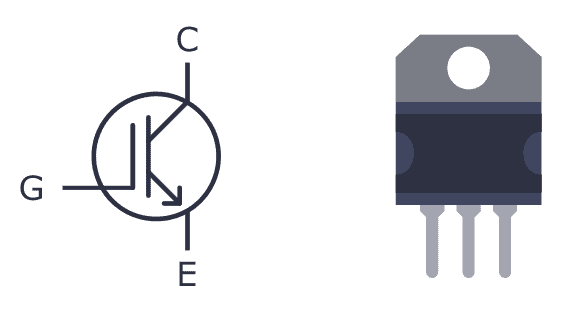
\includegraphics[width=0.45\textwidth]{./images/IGBT.png}
            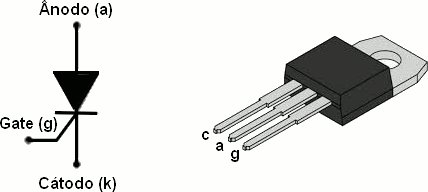
\includegraphics[width=0.45\textwidth]{./images/tiristor.png}
        \caption{À esquerda: IGBT. À direita: Tiristor.}
        \end{figure}
        \subsection{Estrutura do IGBT}

        A célula IGBT é construída semelhante ao MOSFET, porem a mudança está em que a parte n${^+}$ é substituida por uma camada coletora p${^+}$ desse modo forma um transistor PNP vertical, tal região coletora cria uma espécie de conexão do tipo Transistor Bipolar PNP com um MOSFET com a parte n${^+}$ na superfície, juntando assim o "melhor" dos dois dispositivos formando uma estrutura NPNP.

        \subsection{Modelagem matemática e física do IGBT}
        \subsection{Design do componente}
        \subsection{}
        \subsection{}

\section{Conclusões}

    Com este trabalho foi possível compreender de forma mais clara os tipos e funcionalidades dos resistores e capacitores em diferentes circuitos eletrônicos, abordando desde materiais de fabricação dos componentes a casos especiais de aplicações específicas. Com isso evidenciando que a escolha do tipo adequado de componente é parte fundamental na construção de qualquer tipo de circuito, dependendo diretamente das condições de operação do circuito, sendo necessário considerar a tolerância, dissipação de potência, tensão de trabalho, resistência interna do capacitor e estabilidade térmica necessária para cada caso.

    Dessa forma, vemos que os resistores e capacitores não devem ser vistos apenas como elementos básicos em um esquema eletrônico, mas como peças-chave que definem o desempenho, a segurança e a confiabilidade de um projeto. Sua seleção adequada exige não apenas conhecimento técnico, mas também compreensão prática das condições reais de operação.

\newpage

\bibliography{referencia}
\end{document}
